\begin{figure}[H]
    \centering
    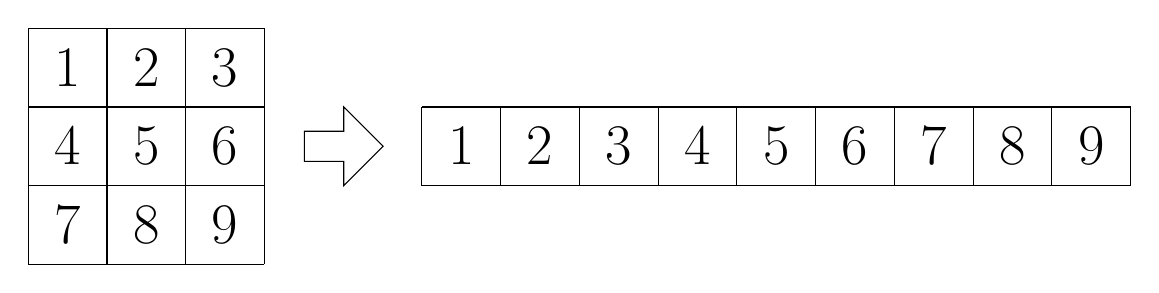
\begin{tikzpicture}
        \usetikzlibrary{shapes.arrows}

        % grid left
        \draw[step=1] (0,0) grid (3,3);
        \node at (.5, 2.5) {\huge 1};
        \node at (1.5, 2.5) {\huge 2};
        \node at (2.5, 2.5) {\huge 3};
        \node at (.5, 1.5) {\huge 4};
        \node at (1.5, 1.5) {\huge 5};
        \node at (2.5, 1.5) {\huge 6};
        \node at (.5, .5) {\huge 7};
        \node at (1.5, .5) {\huge 8};
        \node at (2.5, .5) {\huge 9};

        % arrow
        \node[draw, single arrow,
              minimum height=1cm, minimum width=1cm,
              single arrow head extend=2mm,
              anchor=west] at (3.5,1.5) {};

        % grid right
        \draw[step=1] (5,1) grid (14,2);
        \node at (5.5, 1.5) {\huge 1};
        \node at (6.5, 1.5) {\huge 2};
        \node at (7.5, 1.5) {\huge 3};
        \node at (8.5, 1.5) {\huge 4};
        \node at (9.5, 1.5) {\huge 5};
        \node at (10.5, 1.5) {\huge 6};
        \node at (11.5, 1.5) {\huge 7};
        \node at (12.5, 1.5) {\huge 8};
        \node at (13.5, 1.5) {\huge 9};
    \end{tikzpicture}
    \caption{Flattening, or reshaping, of a 3 by 3 image}\label{fig:flatten}.
\end{figure}